\section{CORA Model} \label{sec:cora}
Based on the information gained during the previous sections we have constructed a model in \gls{cora} capable of producing schedules for the nanosatellite.
The \gls{cora} model takes a set of payloads with some requirements which works as constrains, and other descriptive values, as described in \myref{sec:read_input}, in order to produce a schedule that upholds the specifications.
Such descriptions are fed to the model via our own translator program.\\
The \gls{cora} model is composed of four templates; Processor, Scheduler, Insolation, and PayloadWindow.
They model different aspects of the nanosatellite and its environment, and are all described separately below.\\
The templates Processor and Scheduler, are roughly based on those presented by Bisgaard et al. 2016\cite{gomx3}, but have been modified to fit our context as to handle the added parameters.\\
The model is made to optimise in regards to profit, see \myref{sec:read_input}, this is done as the battery level is rarely a concern\cite{gom_space_conversation}.
We therefore chose the approach where we found the schedule that would yield the highest profit, according to the input specification, while having the battery level in mind.
As \gls{kibam} is pessimistic in the sense that it underestimates the \gls{soc} it would be a good choice to implement.
However due to the complexity of \gls{kibam} and the need for non-linear rates, \gls{cora} is not the right tool for this, therefore we have chosen to model the ideal battery model.\\
Since there is uncertainty in regards to how long it takes to complete some payloads, we chose to assume the worst.
This means that it is likely that more energy will be consumed during simulation than in orbit.\\
When setting the cost rate, see \myref{sec:upp_cora}, the user defined profit is used.
When the user defines the profit, large numbers represents that the payload is more profitable than payloads with with lower profit  values.
In \gls{cora}, when running a query where we extract the best trace, it is defined as the trace with the lowest cost.
Because of this we have to calculate the cost as a function based on the defined profit, how this is done can be seen in \cref{lst:calcCost}.\\
The function \uppVar{calcCost()} calculates the cost rate by subtracting the defined profit from $5$.
However, if the nanosatellite is within a window where another payload can only be performed, the cost rate will be multiplied by two in order to make it more expensive to execute. 
This is done to make it more attractive for the model to chose the payloads that are restricted by a window, versus those that may be executed at any time.

\begin{figure}[h]
	\begin{lstlisting}[language=my_c, caption={Function calcCost(), used for calculating the cost rate}, label=lst:calcCost]
void calcCost() {
	.
	.
	.
	else {runCost = 5 - Profit[active]; return;}
	for (i=0;i < Windows;i++){ 
		if(pen && RunInWindow[i][active] == 0){
			runCost = (5 - Profit[active]) *2;
			return;
		} 
	}
}	
	\end{lstlisting}
\end{figure}


The only query that is run in the \gls{cora} model is the one seen in query \ref{eq:cora_q}.
In this query \uppVar{t\_time} is the accumulated time, and \uppVar{ScheduleLength} is the desired length of the schedule.
This query is run with the trace setting \textit{Best}, meaning it will find the schedule that results in the lowest \textit{cost}, i.e. the highest profit.
Therefore the result of this query is the schedule with the highest profit, and this is what the \gls{smc} model will be build upon.

\begin{equation} \label{eq:cora_q}
E<> t\_time == ScheduleLength
\end{equation}

\subsection{Processor} \label{ssec:cora_pro}
We will describe the Processor template first as it is the base for the entire model.
It models the nanosatellite's processor in the sense that it models when the processor should be idling or executing a payload, as well as consuming power while doing so, as seen in \cref{fig:cora_pro}.\\
The processor template synchronise with the scheduler every time it is ready to execute a payload, the scheduler will then send back a synchronisation if the Processor is allowed to do so.
If it is not allowed to execute the payload it will start idling until a change in its environment occurs, indicated by the synchronisation \uppSync{win?}.
If the Scheduler indicates it is possible to execute the payload, it may be the case that the environment does not allow it, e.g. if the payload is dependant on a window which the nanosatellite is not currently in, the processor will try to select another payload to execute.
If the Scheduler approves and all dependencies are fulfilled, the Processor will transition to \uppLoc{Running} where it will remain for the worst case execution time for the selected payload before it transitions to \uppLoc{Wait} where it will remain for the duration of the payloads deadline.

\begin{figure}[h]
	\centering
	\begin{tikzpicture}
	%Locations
	\node [init] (l0) {$\cup$};
	\node [location] (l1) [right of=l0, xshift=30mm] {$\cup$};
	\node [location] (l2) [right of=l1, xshift=40mm, label={
		[align=left]right:
		\textcolor{name}{ready}
	}] {$\cup$};
	\node [location] (l3) [below of=l1, yshift=-30mm, label={
		[align=right]left:
		\textcolor{name}{Wait}\\
		\textcolor{invariant}{x <= TaskTimes[active][2]}
	}] {};
	\node [location] (l4) [below of=l2, yshift=-30mm, label={
		[align=left]right:
		\textcolor{name}{running}\\
		\textcolor{invariant}{x <= TaskTimes[active][1]}\\
		\textcolor{invariant}{\&\& cost' == runCost}
	}] {};
	\node [location] (l5) [above of=l2, yshift=35mm] {C};
	\node [location] (l6) [above of=l1, yshift=35mm, label={
		[align=left]above:
		\textcolor{name}{Idle}\\
		\textcolor{invariant}{cost' == 5}
	}] {};
	\path[->,black, thick] (l0) edge node [midway, below ][align=center]{\textcolor{update}{mayRun()}} (l1);
	\path[->,black, thick] (l1) edge node [midway, above][align=left]{
		\textcolor{select}{a: int[0,N-1]}\\
		\textcolor{guard}{runnableCount() > 0}\\
		\textcolor{guard}{\&\& runnable[a] == 1}\\
		\textcolor{sync}{ready!}\\
		\textcolor{update}{mayRun(), active = a}} (l2);
	\path[->,black, thick] (l2) edge node [midway, right][align=left]{
		\textcolor{guard}{runnable[active] == 1}\\
		\textcolor{guard}{\&\& !checkBattery()}\\		
		\textcolor{sync}{run?}\\
		\textcolor{update}{updateBattery(), calcCost()}} (l4);
	\path[->,black, thick] (l2) edge[bend right=35] node [midway, left][align=center]{
		\textcolor{sync}{run?}}(l6);
	\path[->,black, thick] (l4) edge node [midway, below][align=center]{
		\textcolor{guard}{x >= TaskTimes[active][1]}} (l3);
	\path[->,black, thick] (l3) edge node [midway, left][align=right]{
		\textcolor{guard}{x >= TaskTimes[active][2]}\\
		\textcolor{update}{reset(), dequeue(),}\\
		\textcolor{update}{x = 0, mayRun()}} (l1);
	\path[->,black, thick] (l1) edge node [midway, left][align=left]{
		\textcolor{guard}{runnableCount() == 0}} (l6);
	\path[->,black, thick] (l6) edge node [midway, above][align=left]{
		\textcolor{sync}{win?}} (l5);
	\path[->,black, thick] (l5) edge node [midway, right][align=left]{
		\textcolor{select}{a: int[0,N-1]}\\
		\textcolor{sync}{ready!}\\
		\textcolor{update}{mayRun(), active = a}} (l2);
	\path[->,black, thick] (l2) edge[bend left=45] node [midway, below][align=center]{
		\textcolor{guard}{runnable[active] == 0}\\
		\textcolor{guard}{\&\& !checkBattery()}\\
		\textcolor{sync}{run?}} (l1);
	\end{tikzpicture}
	\caption{Processor template}
	\label{fig:cora_pro}
\end{figure}

\subsubsection{Scheduler} \label{ssec:cora_sch}
The scheduler always checks if there are enough remaining energy.
When receiving the synchronisation \uppSync{ready?} it will answer back with \uppSync{run!}.
The template is also responsible for deadlocking if the battery \gls{soc} goes below the safety threshold, thereby discarding the current trace which will force it to try another one.
If all traces results in a deadlock it was not possible to produce a schedule with the specified parameters.
The Scheduler template can be seen in \cref{fig:cora_schedule}.

\begin{figure}[H]
	\centering
	\begin{tikzpicture}
	%Locations
	\node [init] (l0) [label={[align=left]left:
		\textcolor{invariant}{checkBattery()}
	}] {};
	\node [location] (l1) [right of=l0, xshift=40mm, label={
		[align=left]right:
		\textcolor{invariant}{checkBattery()}
	}] {$\cup$};
	\path[->,black, thick] (l0) edge[bend left=30] node [midway, above][align=center]{
		\textcolor{sync}{ready?}} (l1);
	\path[->,black, thick] (l1) edge[bend left=30] node [midway, below][align=center]{
		\textcolor{sync}{run!}} (l0);
	\end{tikzpicture}
	\caption{Scheduler template}
	\label{fig:cora_schedule}
\end{figure}

\subsection{Insolation} \label{ssec:cora_ins}
The model consist of two locations \uppLoc{inSun} and \uppLoc{inEclipse}, as seen in \cref{fig:cora_inso}.
The nanosatellite can only recharge when it has a clear line of sight to the sun, which is indicated by the location \uppLoc{inSun}.
The recharging is done on the looping edge on \uppLoc{inSun} with the function \uppUpdate{increaseBattery()}.
This is done four times per orbit, rather than for each time unit, in order to minimise the state space.
When half of the \uppVar{OrbitTime} have passed, modelling the time it takes the nanosatellite to complete one half of its orbit, the model is forced to transition to \uppLoc{inEclipse}.
It is assumed that the nanosatellite always spends exactly half its time in insolation.

\begin{figure}[H]
	\centering
	\begin{tikzpicture}
	%Locations
	\node [init] (l0) [label={
		[align=left]above:
		\textcolor{name}{inSun}
	}, label={
	[align=left]left:
	\textcolor{invariant}{splitTime <= OrbitTime / 8}\\
	\textcolor{invariant}{\&\& ins <= OrbitTime / 2}
}] {};
\node [location] (l1) [right of=l0, xshift=40mm, label={
	[align=left]above:
	\textcolor{name}{inEclipse}
}, label={
[align=left]right:
\textcolor{invariant}{splitTime <= OrbitTime / 8}\\
\textcolor{invariant}{\&\& ins <= OrbitTime / 2}
}] {};
%Edges
\path[->,black, thick] (l0) edge[bend left=30] node [midway, above][align=left]{
	\textcolor{guard}{ins >= OrbitTime / 2}\\
	\textcolor{guard}{\&\& chargeCount == 4}} (l1);
\path[->,black, thick] (l1) edge[bend left=30] node [midway, below][align=left]{
	\textcolor{guard}{ins >= OrbitTime}\\
	\textcolor{guard}{\&\& chargeCount == 8}\\
	\textcolor{update}{ins := 0,}\\
	\textcolor{update}{splitTime = 0}\\
	\textcolor{update}{chargeCount = 0}} (l0);
\path[->,black, thick] (l0) edge [loop below] node [midway, below left][align=left]{
	\textcolor{guard}{splitTime >= OrbitTime/8}\\
	\textcolor{update}{increaseBattery()}} (l0);
\path[->,black, thick] (l1) edge [loop below] node [midway, below right][align=left]{
	\textcolor{guard}{splitTime >= OrbitTime/8}\\
	\textcolor{update}{subIdle()}} (l1);
\end{tikzpicture}
\caption{Insolation template}
\label{fig:cora_inso}
\end{figure}

A few assumptions have been made when this template was modelled, and there is an inaccuracy as we only recharge four times during insolation.
This may result in a suboptimal schedule as executing a payload may cause the \gls{soc} to fall below the threshold, invalidating the trace, where the \gls{soc} should be higher potentially resulting in it being possible to execute the payload.
However, we believe this to be an edge-case that will rarely occur.
In \cref{fig:granularity} we see a graph over the \gls{soc} (left) while doing nothing but charging.
On the right, is a close-up of the same graph.
The blue line shows what the \gls{soc} should be and the orange what it is with our implementation.
Clearly our implementation is not entirely accurate, but neither is the ideal battery model, and because of this we believe a small margin of error is acceptable given the significantly reduced execution time.

\begin{figure}[h]%
	\centering
	\subfloat{{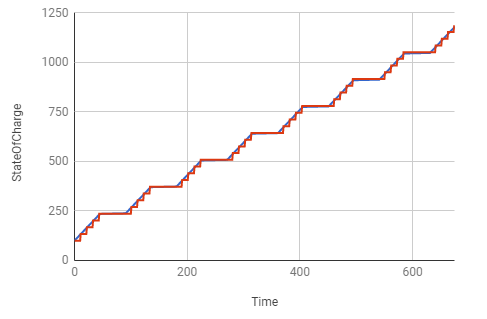
\includegraphics[width=7cm]{graphics/granularity.png} }}
	\qquad
	\subfloat{{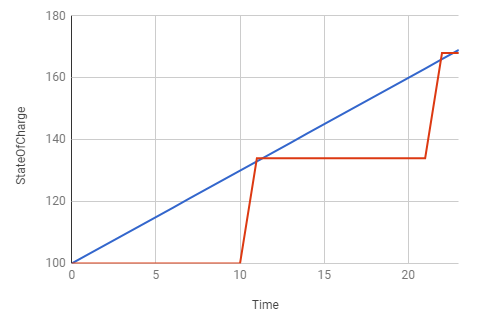
\includegraphics[width=7cm]{graphics/granularity_zoom.png} }}
	\caption{Graphs illustrating \gls{soc}, with different granularity. Bottom graph is a zoom in of the top graph.}
	\label{fig:granularity}%
\end{figure}

To find the effect of execution time reduction we produced $2 * 10$ schedules of 12 hours each, ten with our implementation and ten where recharge was added for every unit of time elapsed.
The differences in time spend to produce these were quite significant and can be seen in \cref{tab:runTimes}.
The worst case when charging every time unit was $138.76\%$ more than when using our implementation.
\begin{table}[H]
	\centering
	\begin{tabular}{lllll}
		& Granularity 1(s)           & Granularity 11(s)          & Time Increase(\%)           &  \\ \cline{2-4}
		\multicolumn{1}{l|}{Best}    & \multicolumn{1}{l|}{39.63} & \multicolumn{1}{l|}{21.13} & \multicolumn{1}{l|}{85.53}  &  \\
		\multicolumn{1}{l|}{Worst}   & \multicolumn{1}{l|}{64.68} & \multicolumn{1}{l|}{27.09} & \multicolumn{1}{l|}{138.76} &  \\
		\multicolumn{1}{l|}{Average} & \multicolumn{1}{l|}{48.13} & \multicolumn{1}{l|}{24.89} & \multicolumn{1}{l|}{93.37}  &  \\ \cline{2-4}
	\end{tabular}
		\caption{Execution times when generating a 12 hour schedule, using different granularity for insolation}
		\label{tab:runTimes}
\end{table}
Our implementation would recharge at time 11, 22, 33 and, 44 as the orbit time were set to 90, which is why the granularity in the second column is set to 11.
Additionally it is assumed that the nanosatellite are always starting in insolation, resulting in our model only being able to produce an accurate schedule for the nanosatellite that matches our starting point.


\subsection{PayloadWindow}\label{ssec:cora_tw}
The last template is the PayloadWindow, this template have one instance for each defined window.
The template is used to model the windows as described in \myref{sec:read_input}.
Windows is an important restriction when producing a schedule as some payloads may be pointless to execute outside of their respective windows.
When a change to a window occurs it will synchronise with the processor on the channel \uppChan{win}, if it is in \uppLoc{Idle} which indicates it may execute some payload.
Otherwise it will transition to the next location updating some variables indicating if the nanosatellite is within the window or not.
A figure of this template can be seen in \cref{fig:cora_window}.\\
It is assumed that an orbit is constant, meaning if the orbit starts whit the nanosatellite over Paris the orbit will also end there.  
